\documentclass[conference]{IEEEtran}
\usepackage[spanish, es-tabla]{babel}
\IEEEoverridecommandlockouts
\usepackage{cite}
\usepackage{amsmath,amssymb,amsfonts}
\usepackage{algorithmic}
\usepackage[table,xcdraw]{xcolor}
\usepackage{graphicx}
\usepackage{subfigure}
\usepackage{textcomp}
\usepackage{xcolor}
\usepackage[hidelinks]{hyperref}
\usepackage{lipsum}
\usepackage{float}
\newtheorem{theorem}{Theorem}
\newtheorem{lemma}{Lemma}

\def\BibTeX{{\rm B\kern-.05em{\sc i\kern-.025em b}\kern-.08em
    T\kern-.1667em\lower.7ex\hbox{E}\kern-.125emX}}
    
\begin{document}

\title{Evaluación de Modelos de Series de Tiempo en Acciones Volátiles}
\author{\IEEEauthorblockN{Alejandra Ossa Yepes}
\IEEEauthorblockA{\textit{Departamento de Ciencias Matemáticas} \\
\textit{Universidad EAFIT}\\
Medellin, Colombia \\
aossay@eafit.edu.co
}

\and

\IEEEauthorblockN{David Plazas}
\IEEEauthorblockA{\textit{Departamento de Ciencias Matemáticas} \\
\textit{Universidad EAFIT}\\
Medellin, Colombia \\
dplazas@eafit.edu.co}
}

\maketitle

\begin{abstract}
Se utiliza la acción financiera de Johnson \& Johnson durante cinco años para realizar un análisis económico con modelos auto-regresivos y una comparación entre ellos, con el fin de generar una discusión de cuál es el más propicio y el que mejor genera una predicción a corto plazo. Se utilizo la herramienta \textit{Rstudio} para calcular cinco modelos cada uno con característica diferentes y obtenidos intuitivamente por medio de un análisis preliminar de la serie, además es importante mencionar que este trabajo tiene un fin académico simplemente exploratorio y que no es el más adecuado para este tipo de modelos. 
\end{abstract}

\begin{IEEEkeywords}
Stock prices, ARIMAX models, GARCH models, identification, validation and forecast of time series data.
\end{IEEEkeywords}

\section{Introducción}
Johnson \& Johnson (JNJ) es una compañía de 132 años, que se especializa en productos farmacéuticos, cuidado de la salud del consumidor y dispositivos médicos, vende una amplia gama de productos de salud y belleza que incluyen la línea Johnson's Baby, Neutrogena, Listerine, Band Aids, Tylenol y Motrin. En Estados Unidos por ingresos brutos fue la empresa número 37 según el índice Fortune 2018 \cite{fortune2018}. La acción financiera de esta entidad ha sido fuertemente golpeada por diferentes sucesos en la última década, por lo que se presenta diversos comportamientos en la acción financiera de la compañía.  

Debido al problema de salud pública actual, las entidades farmacéuticas han hecho una carrera contra el reloj por destacarse dentro de su ámbito y tener un reconocimiento mundial por su participación, siendo así que JNJ ha sido una de las compañías promotoras de estudios sobre esta enfermedad estando así en la mirada de todos con sus últimas declaraciones de la creación de una vacuna, por tal motivo realizar un análisis económico del comportamiento de las acciones de esta compañía es de gran interés. Para este trabajo, se dispuso de las herramientas ofrecidas por las series de tiempo para estimar modelos que describan el comportamiento  financiero de la empresa y finalmente realizar predicciones sobre ellas. El documento presenta un análisis preliminar de las características que contiene la serie de tiempo y las posibles dificultades que se pueden presentar con la estimación de los modelos, entre estas, la secuencialidad en la serie. Para esto, se optó por un análisis semanal, separando los datos por días de la semana, pero no se obtuvieron resultados favorables. 

En este documento se usaron 5 variados modelos de estimación los cuales tienen como fin realizar una diversificación de los modelos y por último una comparación de cuál es el más propicio para la serie, cabe aclarar que cada uno de estos modelos cuenta con su respectiva validación y por último una predicción a corto plazo. 

\section{Metodología e Identificación}
Se utilizó un enfoque inductivo para la identificación de los diferentes modelos propuestos para el precio de cierre de la acción de JNJ, puesto que se enfocó en hacer extensas experimentaciones para identificar factores clave, previo a decidir qué tipo de modelo o proponer alguno basado en la teoría o literatura.

Cabe resaltar que se cuentan con 1259 datos extraídos directamente de \href{https://finance.yahoo.com}{\textit{Yahoo Finance}} el día 30 de Octubre de 2020; por otra parte, los datos son los precios de cierre diarios de la acción de JNJ desde el 2 de Noviembre de 2015 (cinco años). Nótese que los precios sólo se obtienen para días laborales, no se cuentan con datos de fines de semana ni festivos. Es por este motivo que la serie no tiene secuencialidad a través del tiempo. Para fines de este trabajo, se asume que estos datos pueden considerarse secuenciales. Adicionalmente, la metodología y los procesos para el desarrollo de este trabajo están basados en los aprendizajes desarrollados en la materia y los seguimientos; no obstante se recurrió a \cite{uriel1985}, \cite{tsay2005analysis} y \cite{shumway2017time} como fuentes bibliográficas para corroborar resultados. Todo el código para el desarrollo de este proyecto se puede encontrar en el \href{https://github.com/Daples/daples/tree/master/time-series/src}{\textit{repositorio de GitHub}} de uno de los autores.

\subsection{Análisis Preliminar}
La gráfica de la serie de tiempo, bajo el supuesto de secuencialidad, se puede observar en la Figura \ref{fig:ts}. Nótese que la serie inmediatamente da indicios de no estacionariedad, al tener una aparente tendencia de crecimiento en los últimos cinco años. También se puede observar un comportamiento atípico a comienzos del 2020, esto es dado a la contingencia global causada por el SARS-CoV2, pues al rededor de esta fecha se declaró como pandemia.

\begin{figure}
    \centering
    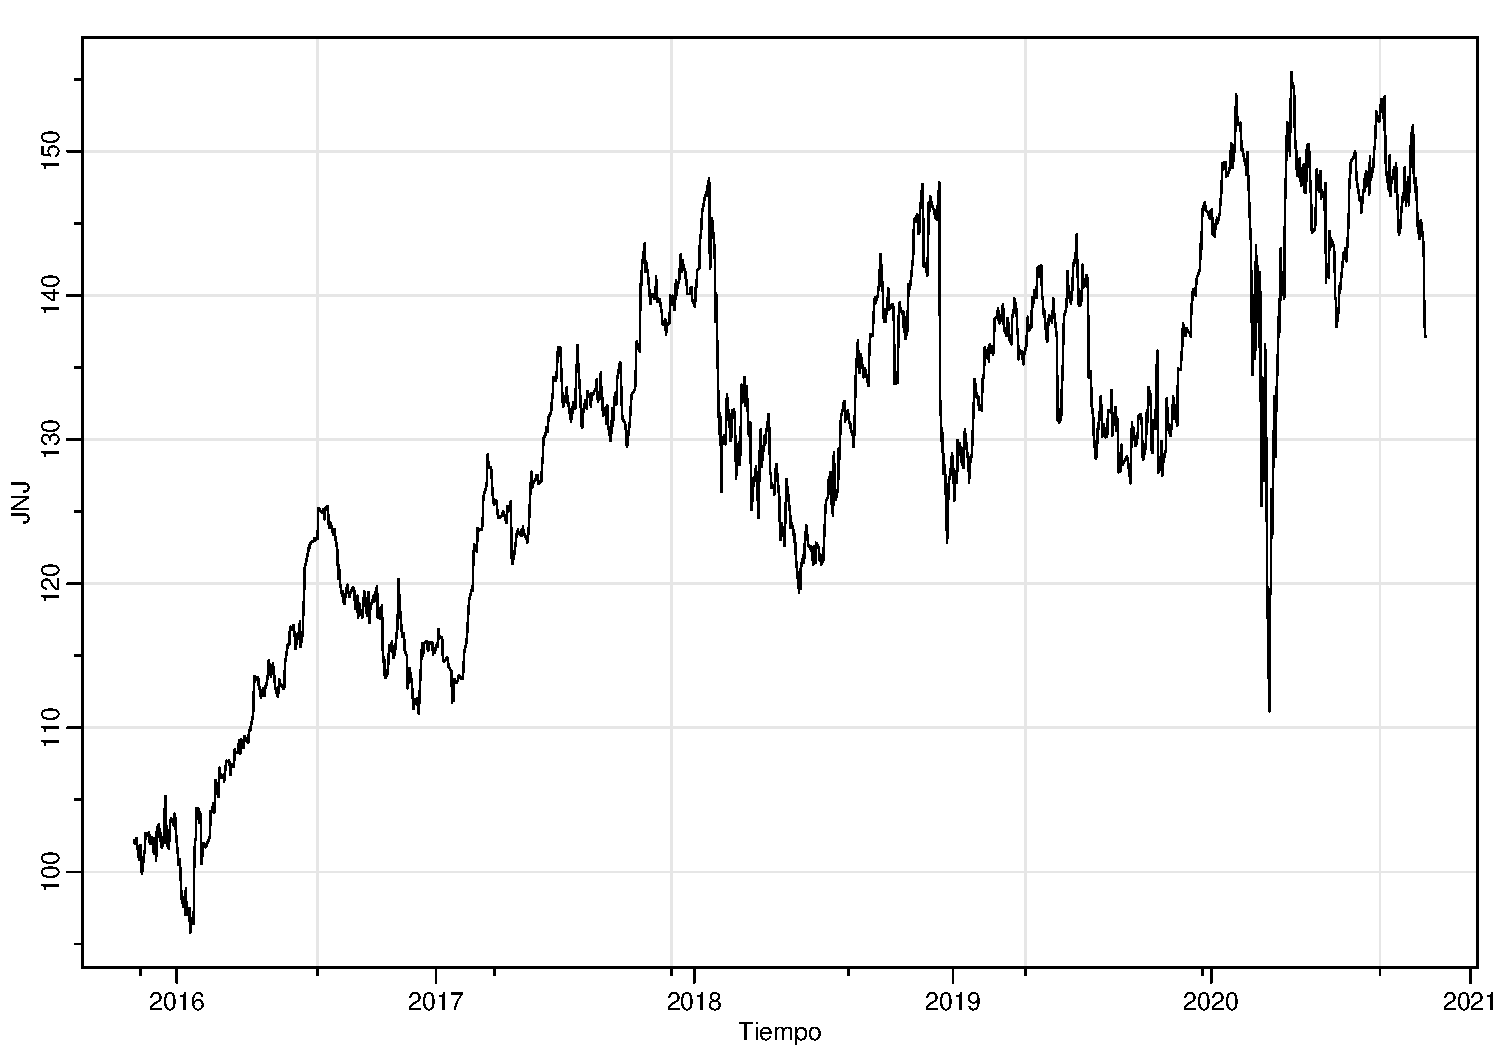
\includegraphics[width=\columnwidth]{figs/ts.pdf}
    \caption{Serie de tiempo.}
    \label{fig:ts}
\end{figure}

Es importante mencionar que los datos de acá en adelante son considerados hasta el comienzo de Septiembre de 2020, con el objetivo de dividir la muestra en un conjunto de ``entrenamiento'' (ajuste de los parámetros) y otro para hacer validación ``in-sample'', para evaluar el ajuste del modelo a los datos reales. Adicionalmente, los diagramas de autocorrelación de la serie de tiempo, tanto el total como el parcial, se muestran en la Figura \ref{fig:acf_og}. Obsérvese que la autocorrelación es alarmantemente elevada y la parcial no muestra comportamientos significativos después del primer lag. Estos dos factores sugieren que el proceso cuenta con una raíz unitaria, pues son características usuales en procesos como el paseo aleatorio.

\begin{figure}
    \centering
    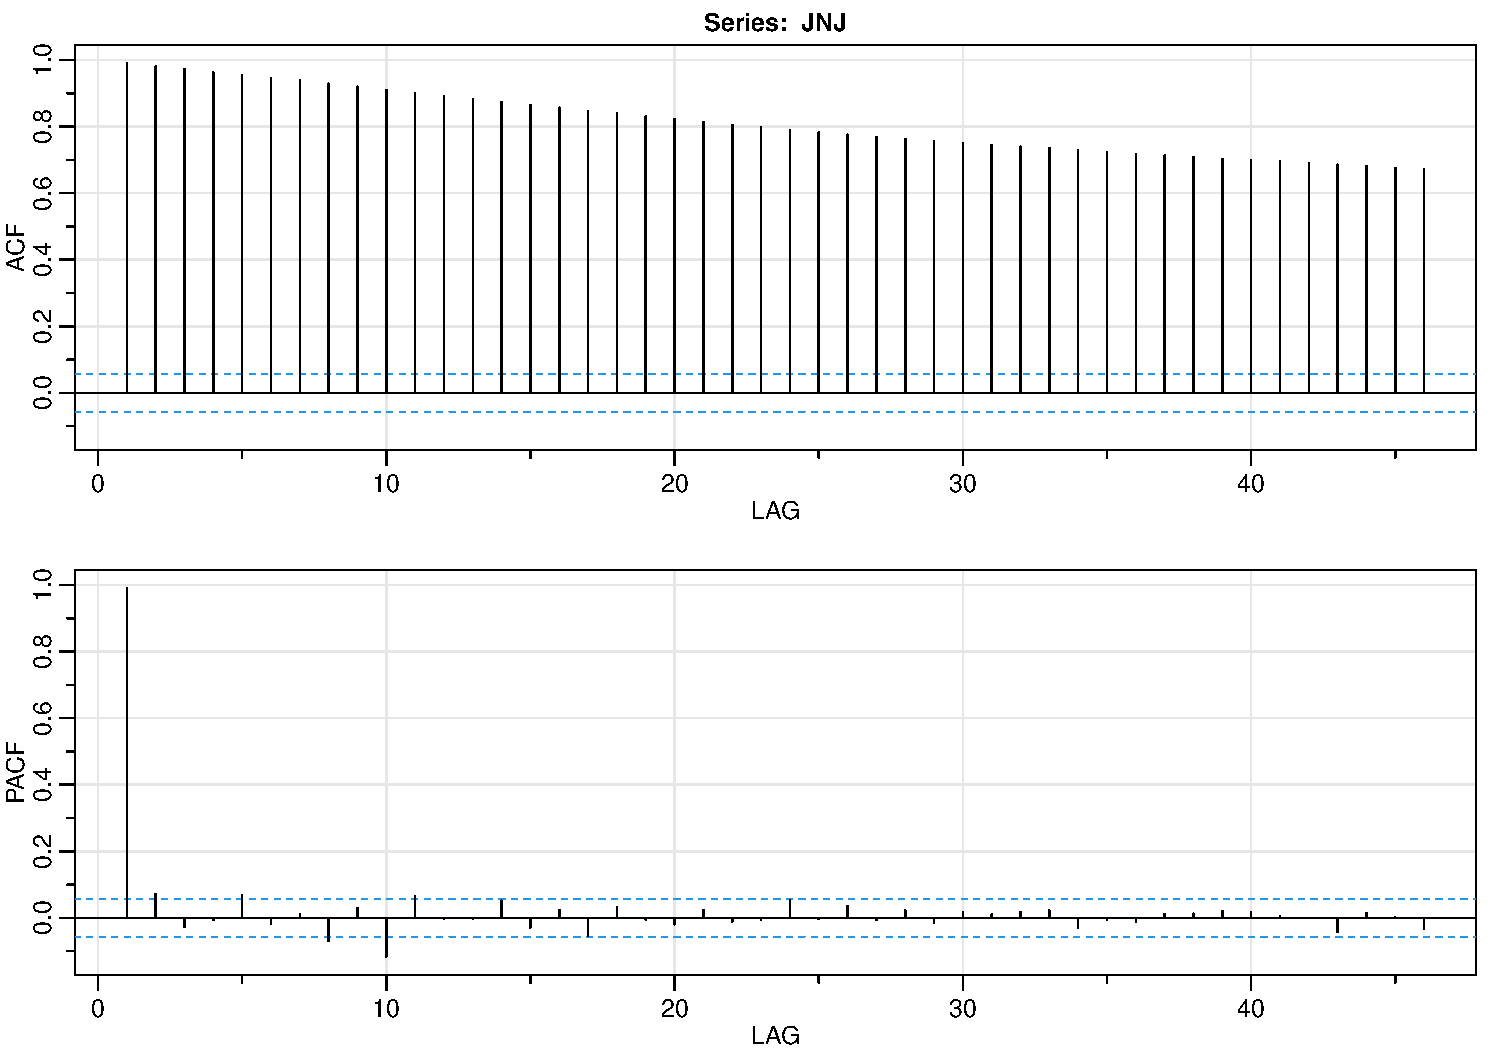
\includegraphics[width=\columnwidth]{figs/acf_og.pdf}
    \caption{Diagramas de autocorrelación.}
    \label{fig:acf_og}
\end{figure}

Para corroborar esta hipótesis, se hicieron los tests de Dickey-Fuller Aumentado (ADF) y el Kwiatkowski–Phillips–Schmidt–Shin (KPSS). Estos tests fueron directamente utilizados de R. Los resultados de los tests para la serie de tiempo original se pueden ver en la Tabla \ref{tab:estac_og}.

\begin{table}[H]
\centering
\caption{Tests de estacionariedad para serie original.}
\label{tab:estac_og}
\begin{tabular}{cc}
\hline
\textbf{Test} & \textbf{Valor-P} \\ \hline
ADF & 0.8414 \\
KPSS & $<$0.01 \\ \hline
\end{tabular}
\end{table}

Considerando que la hipótesis nula del ADF es que el modelo tiene una raíz unitaria, y del KPSS es que el modelo es integrado de orden 0, se ve que para ambos tests hay evidencia suficiente de que la serie de tiempo es no estacionaria. Para corregir este comportamiento, la primera diferencia de la serie será tomada. La gráfica de la serie de tiempo después de tomar la primera diferencia se presenta en la Figura \ref{fig:ts_diff}, y los diagramas de autocorrelación total y parcial en la Figura \ref{fig:acf_diff}.

\begin{figure}
    \centering
    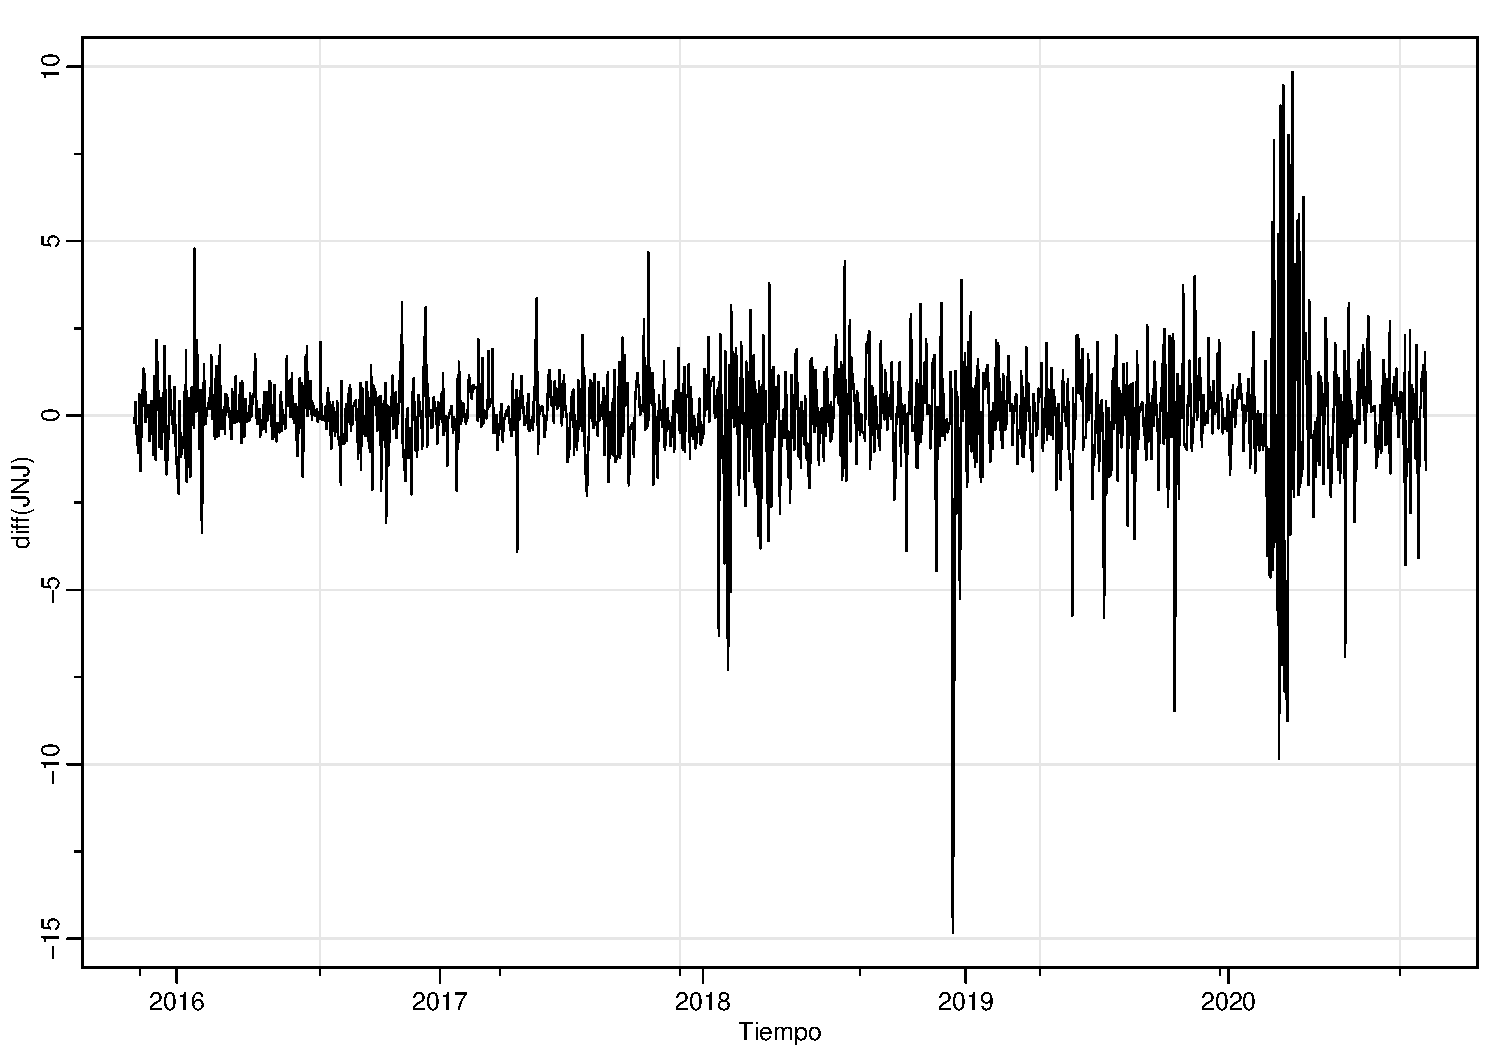
\includegraphics[width=\columnwidth]{figs/ts_diff.pdf}
    \caption{Serie de tiempo diferenciada.}
    \label{fig:ts_diff}
\end{figure}

\begin{figure}
    \centering
    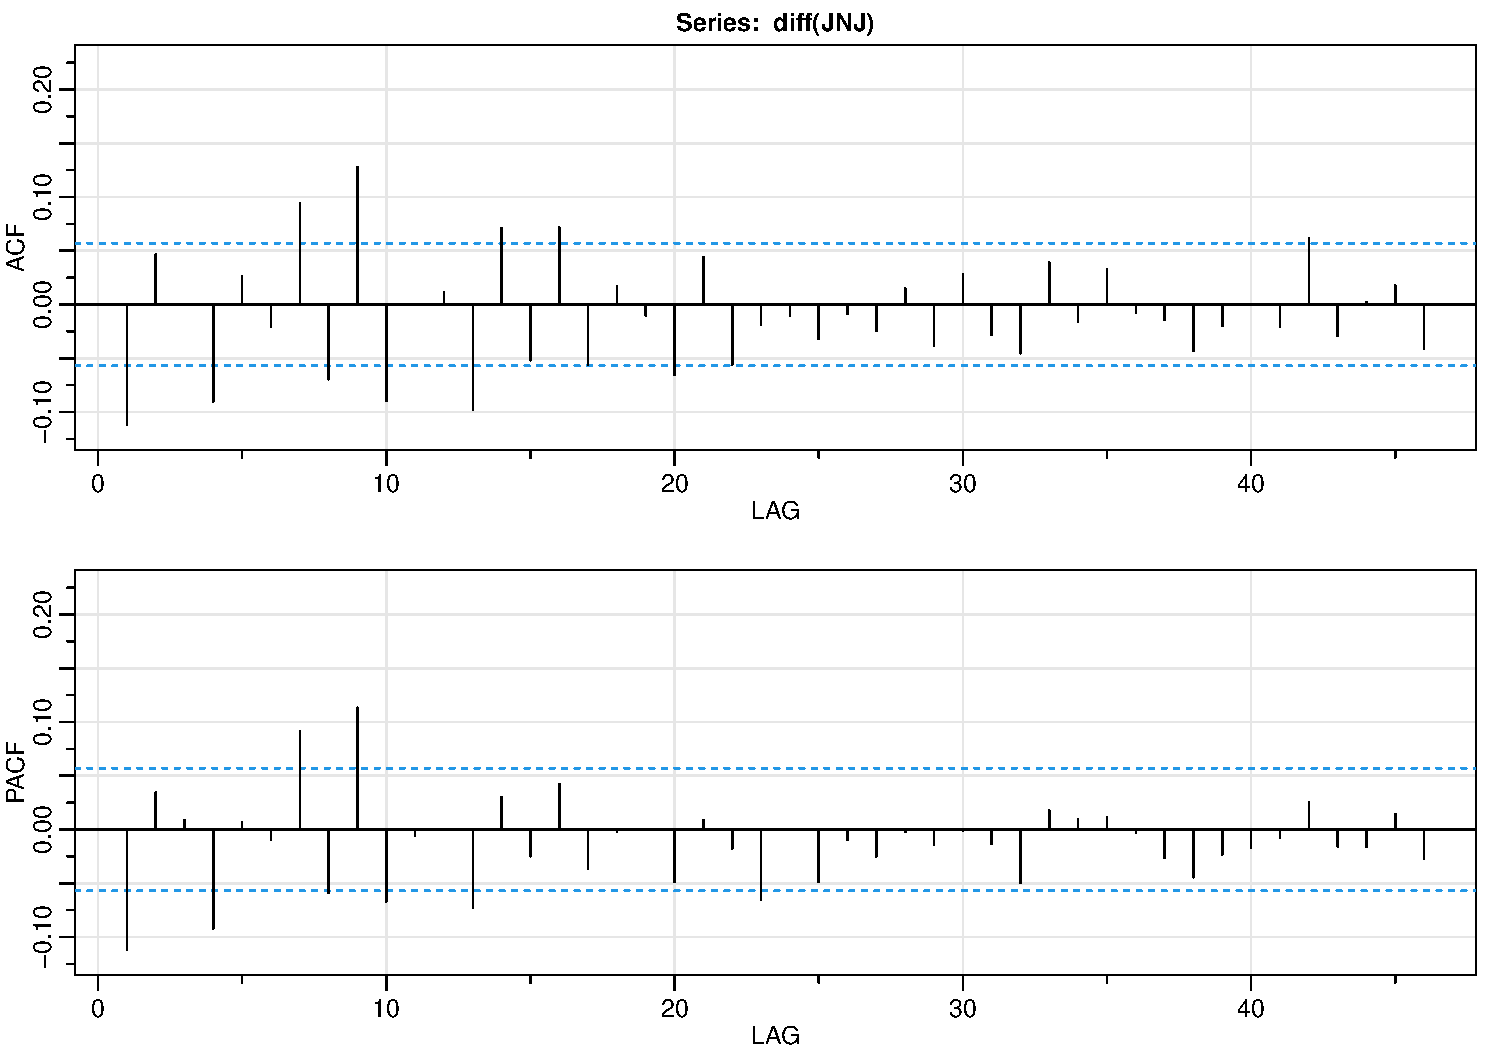
\includegraphics[width=\columnwidth]{figs/acf_diff.pdf}
    \caption{Diagramas de autocorrelación.}
    \label{fig:acf_diff}
\end{figure}

Obsérvese que la serie aparenta tener un comportamiento estacionario, centrado en 0, con alta volatilidad debido a los pronunciados saltos que presenta. Por otra parte, los diagramas de autocorrelación muestran comportamientos más razonables, muy diferentes a los que se mostraron en la serie original. Es importante notar que estos diagramas de autocorrelación no muestran comportamientos usuales, como el decaimiento exponencial o abrupto de la correlación - típicos en modelos AR y MA -, por lo que la identificación del proceso se dificulta. La estacionariedad del modelo fue retesteada para la serie diferenciada, obteniendo los valores-P mostrados en la Tabla \ref{tab:estac_diff}. Obsérvese que en este caso ambos casos afirman que existe evidencia suficiente de estacionariedad en la serie. Basado en este hecho, se estimó el primer parámetro de los modelos tipo $\mathrm{ARIMA}(p,d,q)$ como $d=1$.

\begin{table}[H]
\centering
\caption{Tests de estacionariedad para serie diferenciada.}
\label{tab:estac_diff}
\begin{tabular}{cc}
\hline
\textbf{Test} & \textbf{Valor-P} \\ \hline
ADF & 0.00041 \\
KPSS & $>$0.1 \\ \hline
\end{tabular}
\end{table}

\subsection{Análisis Semanal}
Dado que la serie de tiempo no es propiamente secuencial, también se incluyó un análisis para cada día de la semana. Los datos fueron separados para cada día de la semana y el mismo análisis previo se desarrolló: todas las series de tiempo obtenidas son estacionarias después de 1 diferencia.

Luego, se siguió un proceso de identificación utilizando el comando auto.arima de R. De estos resultados, sólo el modelo para los días Lunes dio un resultado razonable, pues los mejores ARIMA estimados por el programa fueron de orden (0,1,0) para los días Martes, Miércoles, Jueves y Viernes. Es claro que un modelo $\mathrm{ARIMA}(0,1,0)$ es equivalente a un paseo aleatorio, por lo que no fueron considerados dentro de este trabajo. Para incluir un componente semanal, se consideraron variables binarias exógenas dentro de modelos ARIMAX, pero esto será mejor expuesto posteriormente.

\subsection{Identificación}
Los modelos AutoRegresivos Integrados de Medias Móviles (ARIMA, en inglés) son una muy buena aproximación al modelado dinámico de variables económicas en términos de relaciones lineales con su pasado y comportamientos no observables. En general, los modelos ARIMA son suficientes para representar un proceso generador de datos (o al menos aproximarlo en cortos horizontes de tiempo) con fines de análisis y pronóstico; además, los modelos ARIMA son el pilar para la construcción de modelos dinámicos más complejos.

Sea $\{x_t\}_{t\geq0}$ un proceso estocástico en tiempo discreto, se dice éste puede ser modelado por un $\mathrm{ARIMA}(p,d,q)$ si puede ser escrito como
\begin{equation}\label{eq:arima_lag}
    \left(1-\sum_{r=1}^p\phi_rL^r\right)(1-L)^dx_t=\left(1-\sum_{r=1}^q\theta_rL^r\right)\epsilon_t,
\end{equation}
donde $Lx_t:=x_{t-1}$ y con $\phi_r\in\mathbb{R}$, $\theta_r\in\mathbb{R}$, $p,d,q\in\mathbb{N}$ y $\{\epsilon_t\}_{t\geq0}$ un proceso de innovación con varianza $\sigma^2_\epsilon>0$. El modelo de la ecuación (\ref{eq:arima_lag}) puede ser reescrito de forma más intuitiva como 
\begin{equation}
    w_t=\sum_{r=1}^p\phi_rw_{t-r}+\epsilon_t-\sum_{r=1}^q\theta_r\epsilon_{t-r},
\end{equation}
donde $w_t:=(1-L)^dx_t$ es la serie diferenciada para efectos de estacionariedad.

Dada la presencia de picos de autocorrelación en altos rezagos, sin presencia de caída exponencial previa, también podría interpretarse como un modelo con componente estacional (SARMA, en inglés). Un proceso $\{x_t\}_{t\geq0}$ puede modelarse como un modelo $\mathrm{ARIMA}(p,d,q)\times\mathrm{SARMA}(P,Q)_s$ si satisface
\begin{equation}
    \phi(L)\varphi(L^s)(1-L)^dx_t=\theta(L)\vartheta(L^s)\epsilon_t
\end{equation}
donde
\begin{align*}
    \phi(L)&=1-\sum_{r=1}^p\phi_rL^r\\
    \varphi(L^s)&=1-\sum_{r=1}^P\varphi_rL^{rs}\\
    \theta(L)&=1-\sum_{r=1}^q\theta_rL^r\\
    \vartheta(L^s)&=1-\sum_{r=1}^Q\vartheta_rL^{rs}
\end{align*}
y $s$ es el periodo estacional. La forma alternativa de escribir estos modelos es mucho más compleja que la de los modelos ARIMA, pero cabe resaltar que esta expansión permite expresar un modelo $\mathrm{ARIMA}(p,d,q)\times\mathrm{SARMA}(P,Q)_s$ como un simple $\mathrm{ARIMA}(p+Ps,d,q+Qs)$.

Adicionalmente, como se mencionó en la sección anterior, se buscó también incluir componentes exógenas (por días de la semana) en el modelo. Para esto, se utilizaron modelos $\mathrm{ARIMAX}(p,d,q)$ con componente exógena multivariable. Formalmente, este modelo propuesto tiene forma 
\begin{equation}
    w_t=\sum_{r=1}^p\phi_rw_{t-r}+\sum_{r=1}^5\beta_rd_t^r+\epsilon_t-\sum_{r=1}^q\theta_r\epsilon_{t-r},
\end{equation}
donde $w_t=x_t-x_{t-1}$, y la variable $d_t^r\in\{0,1\}$ es una variable binaria (``dummy'') que toma el valor de 1 si el día de la semana correspondiente a $t$ es $r$. Por ejemplo, si $t$ corresponde al día Martes, entonces $d_t^2=1$ y $d_t^r=0$ para $r\neq 2$. Es claro que $r=1$ es Lunes y $r=5$ es Viernes.

Finalmente, dado que estamos trabajando con el precio de una acción financiera, es bien sabido que los modelos generales autoregresivos de heterocedasticidad condicional (GARCH) son más apropiados para modelar esos procesos, dada la alta volatilidad, choques y cambios en la varianza del proceso \cite{ruppert2011}. La idea general de estos procesos es modelar la varianza del proceso, en lugar de la media (como es el caso de los modelos ARIMA).

Un modelo $\mathrm{ARIMA}(p,d,q)/\mathrm{GARCH}(p_G, q_G)$ es una generalización del ARIMA convencional, donde el ruido no es modelado por un proceso de innovación $IID(0,\sigma^2_\epsilon)$, sino que el ruido es modelado directamente a partir del proceso GARCH. Formalmente, se tiene un $\mathrm{ARIMA}(p,d,q)$
\begin{equation}
    w_t=\sum_{r=1}^p\phi_rw_{t-r}+u_t-\sum_{r=1}^q\theta_ru_{t-r},
\end{equation}
donde $\{u_t\}_{t\geq0}$ es un $\mathrm{GARCH}(p_G, q_G)$
\begin{align*}
    u_t&=\sigma_t\epsilon_t,\\
    \sigma_t^2&=\mathbb{E}\left[u^2_t|\Omega_{t-1}\right]\\
    &=\alpha_0+\sum_{r=1}^{p_G}\delta_r\sigma^2_{t-r} + \sum_{r=1}^{q_G}\alpha_ru^2_{t-r}.
\end{align*}

\section{Resultados}
\subsection{Estimación}
\subsubsection{Modelos ARIMA}
En el caso particular de la serie trabajada, ya se discutió que la identificación por las funciones de autocorrelación es compleja, debido a la falta de patrones ``usuales''. De la Figura \ref{fig:acf_diff} puede observarse que ambas funciones tienen picos en noveno lag, lo que podría sugerir la presencia de rezagos de orden 9 significativos tanto para el AR como el MA. Por lo tanto, el primer modelo intuitivo propuesto para la serie de tiempo es un $\mathrm{ARIMA}(9,1,9)$, cuyos coeficientes se presentan en la Tabla \ref{tab:coefs_ar9}. Este modelo tuvo un Criterio de Información de Bayes (BIC) de 4792.84.

\begin{table}[H]
\centering
\caption{Coeficientes $\mathrm{ARIMA}(9,1,9)$.}
\label{tab:coefs_ar9}
\begin{tabular}{ccc}
\hline
\textbf{Lag} & \textbf{AR} & \textbf{MA} \\ \hline
1 & -0.44 & 0.36 \\
2 & 0.09 & -0.10 \\
3 & -0.44 & 0.46 \\
4 & -1.07 & 0.96 \\
5 & -0.44 & 0.35 \\
6 & -0.05 & 0.07 \\
7 & -0.05 & 0.08 \\
8 & -0.52 & 0.43 \\
9 & -0.23 & 0.28 \\ \hline
\end{tabular}
\end{table}

Este modelo se comparó con el otorgado por el comando auto.arima de R, cuyo objetivo es estimar el mejor modelo ARIMA que se ajusta a los datos utilizando el criterio de información para la jerarquía. El mejor modelo, de acuerdo a este proceso, es un $\mathrm{ARIMA}(3,1,2)$ cuyo BIC es de 4733.23. Es claro que el modelo que tenga menor criterio de información es mejor, por esto, desde los modelos ARIMA se seleccionó el (3,1,2) como candidato a la validación. Los coeficientes del modelo estimado se presentan en la Tabla \ref{tab:coefs_arima}.

\begin{table}[H]
\centering
\caption{Coeficientes $\mathrm{ARIMA}(3,1,2)$.}
\label{tab:coefs_arima}
\begin{tabular}{ccc}
\hline
\textbf{Lag} & \textbf{AR} & \textbf{MA} \\ \hline
1 & -1.75 & 1.66 \\
2 & -0.90 & 0.79 \\
3 & -0.01 & $\times$ \\\hline
\end{tabular}
\end{table}
\subsubsection{Modelo ARIMAxSARMA}
Razonando de la misma forma, de la Figura \ref{fig:acf_diff} se puede observar el ``spike'' en el rezago 9, pero sin presencia de autocorrelaciones muy significativas en los rezagos anteriores. Por esto, se pensó en estimar un modelo $\mathrm{ARIMA}(0,1,9)\times\mathrm{SARMA}(1,0)_9$. Los resultados de la estimación en R se presentan la Tabla \ref{tab:coefs_sarma}

\begin{table}[H]
\centering
\caption{Coeficientes $\mathrm{ARIMA}(0,1,9)\times\mathrm{SARMA}(1,0)_9$.}
\label{tab:coefs_sarma}
\begin{tabular}{ccc}
\hline
\textbf{Lag} & \textbf{MA} & \textbf{SAR} \\ \hline
1 & -0.108 & 0.626 \\
2 & 0.001 & $\times$ \\
3 & -0.003 & $\times$ \\
4 & -0.108 & $\times$ \\
5 & 0.027 & $\times$ \\
6 & -0.03 & $\times$ \\
7 & 0.052 & $\times$ \\
8 & -0.061 & $\times$ \\
9 & -0.562 & $\times$ \\
Const. & 0.0372 & $\times$ \\ \hline
\end{tabular}
\end{table}

\subsubsection{Modelo ARIMAX}
El modelo ARIMAX en R sólo pudo modelarse incluyendo 4 de las 5 variables binarias, por razones aun desconocidas para los autores. Los coeficientes del modelo se muestran en la Tabla \ref{tab:coefs_arimax}.

\begin{table}[H]
\centering
\caption{Coeficientes modelo ARIMAX(3,1,2).}
\label{tab:coefs_arimax}
\begin{tabular}{cccc}
\hline
\textbf{Lag} & \textbf{AR} & \textbf{MA} & \textbf{xreg} \\ \hline
1 & -0.885 & 0.780 & -0.165 \\
2 & -0.909 & 0.857 & 0.064 \\
3 & -0.047 & $\times$ & 0.104 \\
4 & $\times$ & $\times$ & 0.030 \\ \hline
\end{tabular}
\end{table}

\subsection{Validación}
El objetivo de la validación  es encontrar el modelo más  adecuado para la representación de la serie estudiada, por lo que se analizar los elementos que debe cumplir un modelo para que sea ideal.

\subsubsection{Ruido blanco} Para el análisis residual de los errores estimados de cada uno de los modelos, se puede evidenciar rechazo de la hipótesis nula tanto el test Box-Ljung como el Box-Pierce presentada en la Tabla \ref{tab:tablaruidob} demostrando no autocorrelación en los errores estimados.
\begin{table}[H]
\centering
\caption{No autocorrelación de los residuales de los modelos }
\label{tab:tablaruidob}
\begin{tabular}{ccc}
\hline
\textbf{Modelos} & \textbf{Box-Ljung} & \textbf{Box-Pierce} \\ \hline
ARMA(9,1,9) & 0.989 & 0.989 \\
ARMA(0,1,9)$\times$SARMA(1,0) & 0.581 & 0.581 \\
ARIMA(3,2,1) & 0.978 & 0.978 \\
ARIMAX(3,2,1) & 0.994 & 0.994 \\
GARCH(1,1)/ARMA(1,0) & 0.078 & 0.079 \\ \hline
\end{tabular}
\end{table}

\subsubsection{Estacionariedad y Estabilidad} Para analizar el problema de estacionaridad se busca factorizar el polinomio de la parte autoregresiva de cada uno de los modelos y observar si $\hat{\lambda_{i}}$ es cercano a 1 para tener indicios de no estacionaridad de la serie, igualmente  para la parte MA se  factoriza las raíces y se observar que $\hat{\delta}_{i}$ sea lejano de 1 para garantizar invertibilidad del modelo.

\begin{figure}
    \centering
    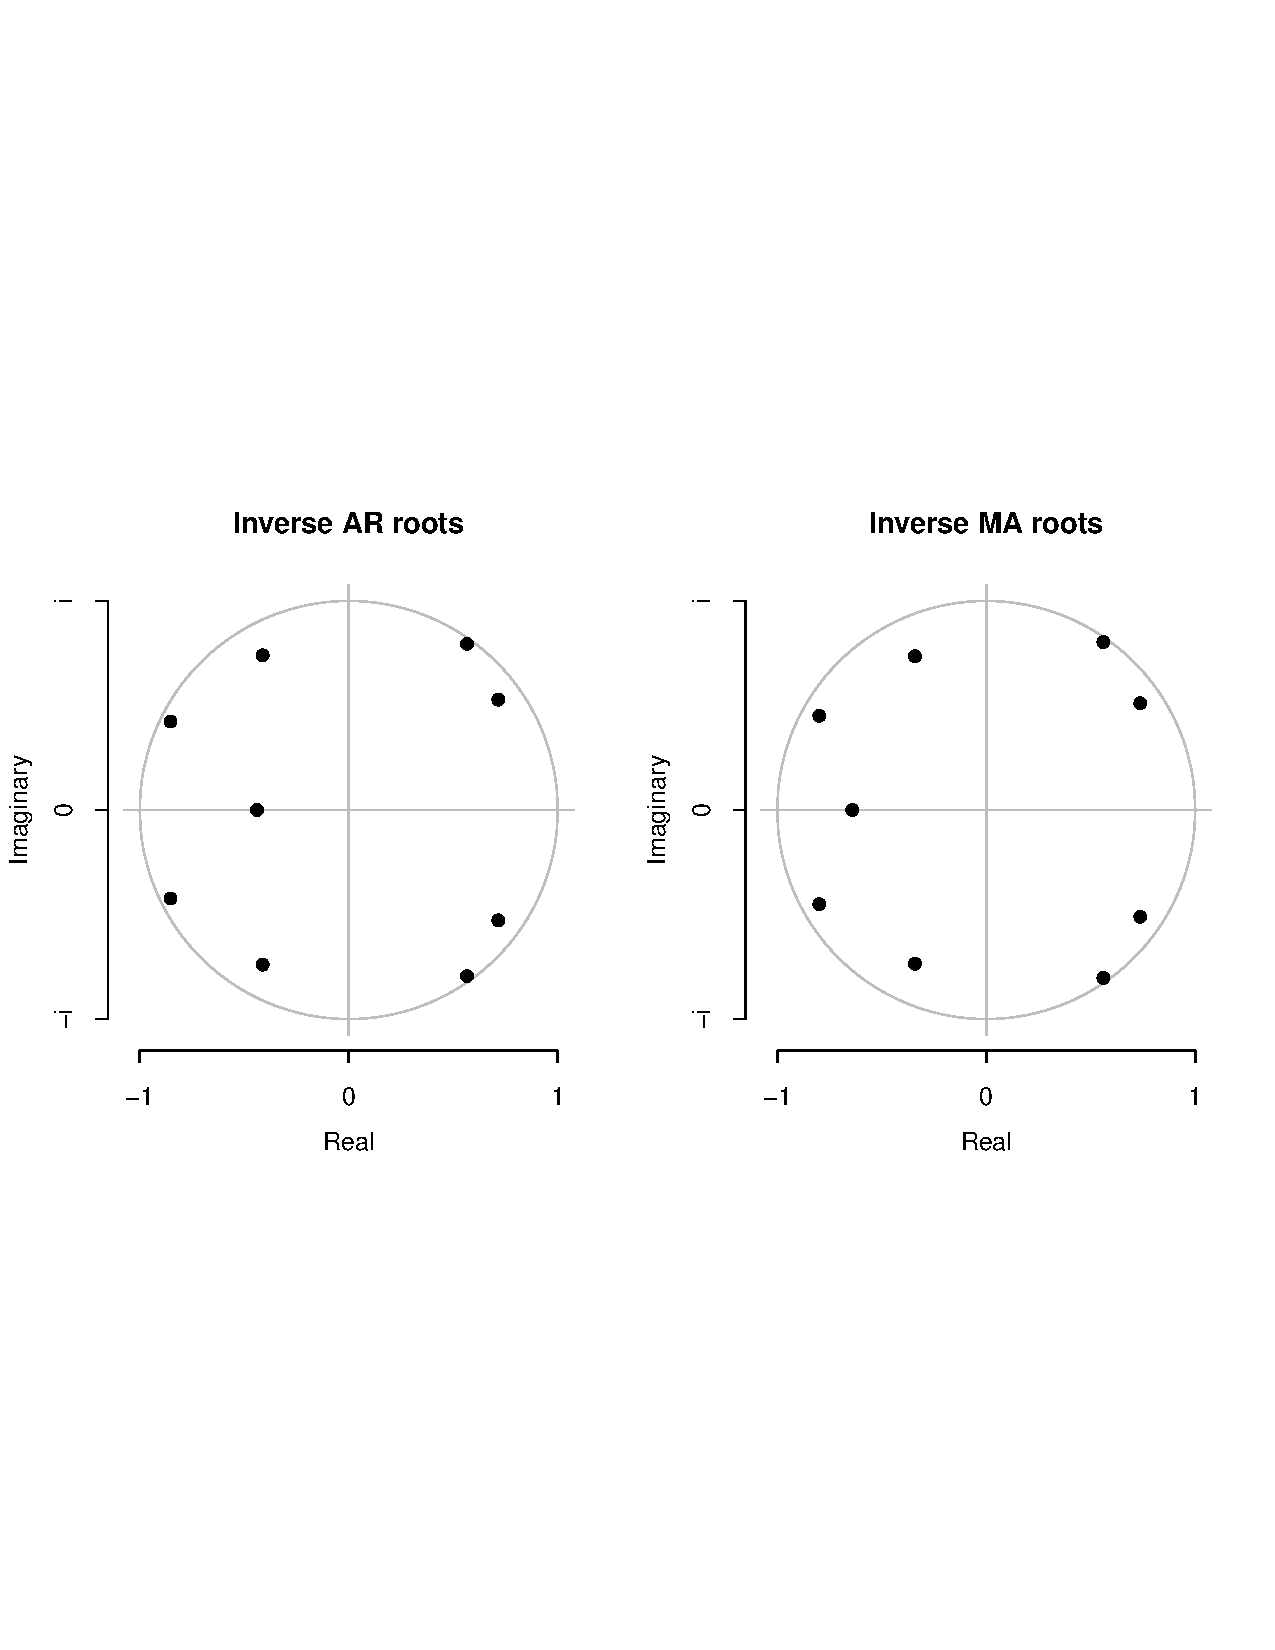
\includegraphics[width=\columnwidth]{figs/AR9stationary.pdf}
    \caption{Lugar de las raíces para el ARIMA(9,1,9).}
    \label{fig:Inverti1}
\end{figure}

\begin{figure}
    \centering
    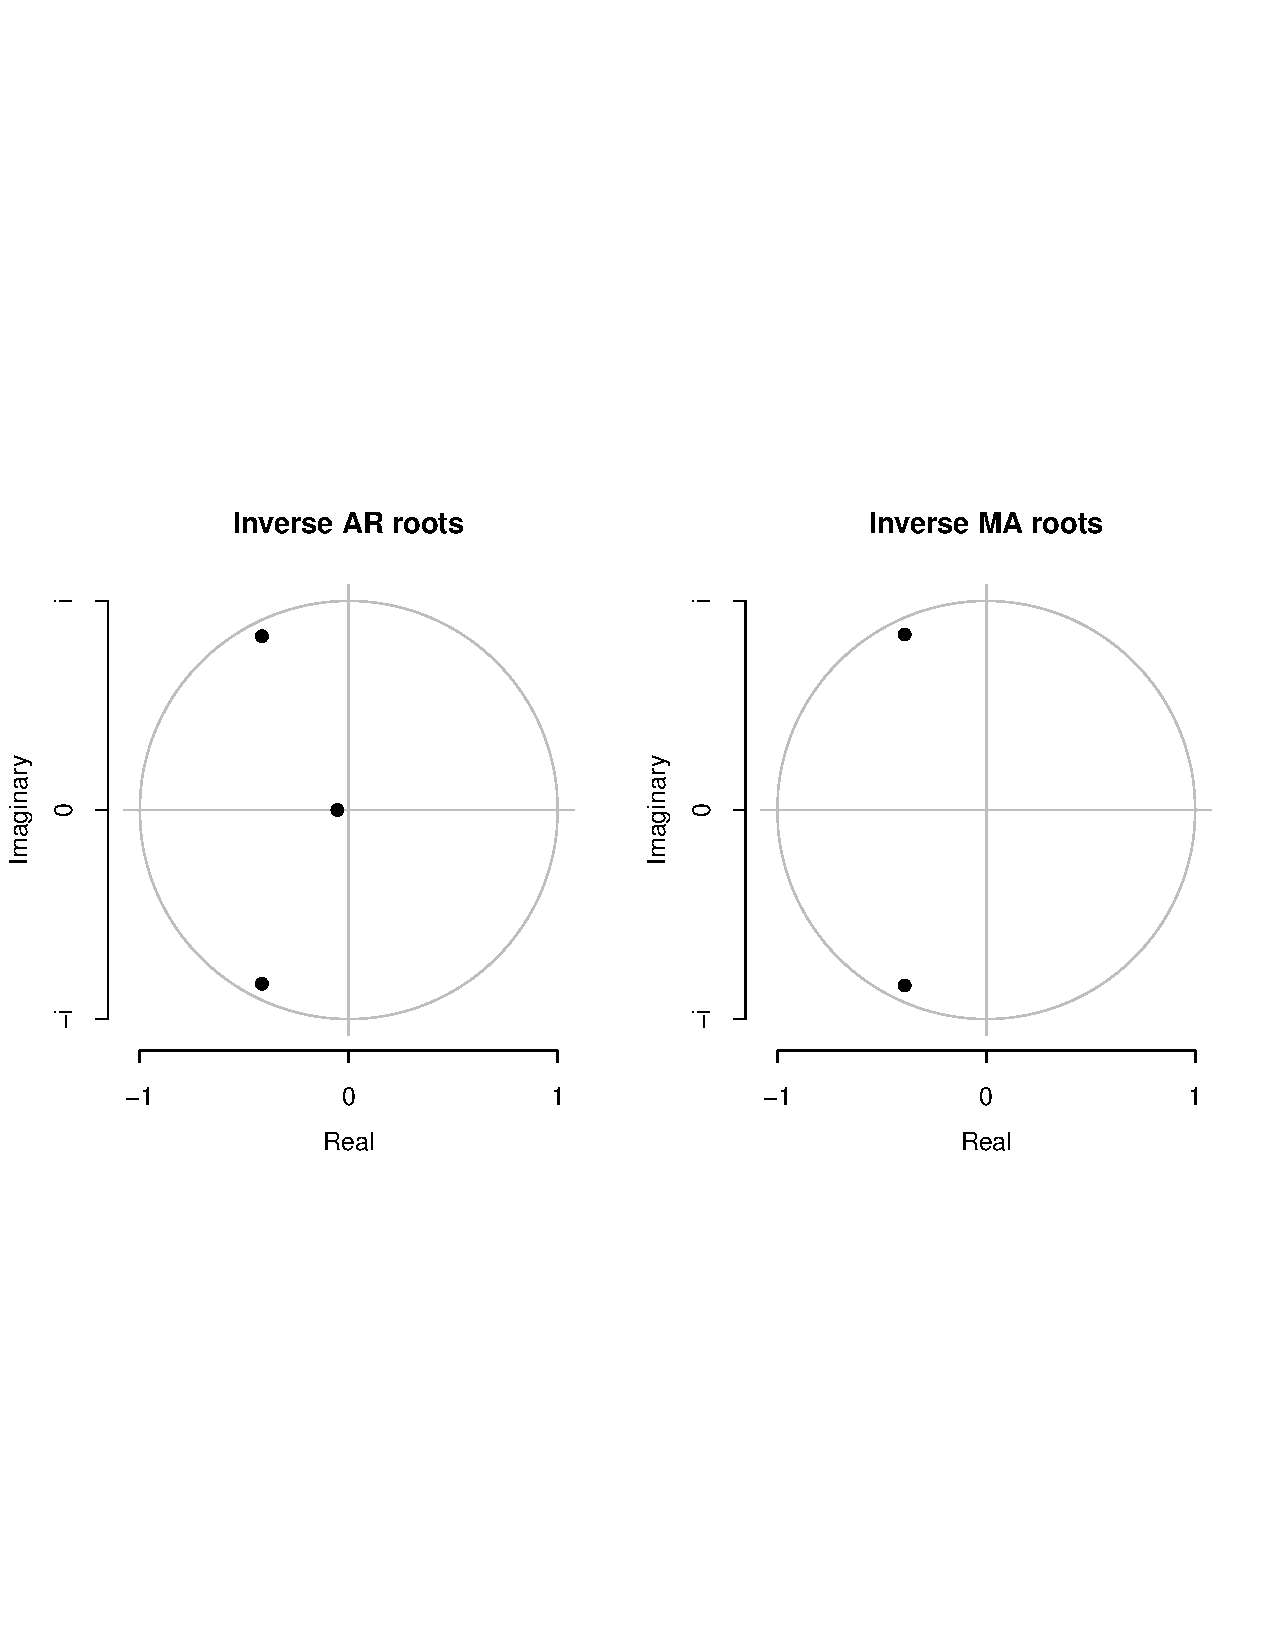
\includegraphics[width=\columnwidth]{figs/Arimaxstationary.pdf}
    \caption{Lugar de las raíces para el ARIMAX(3,1,2).}
    \label{fig:Inverti2}
\end{figure}

\begin{figure}[t]
    \centering
    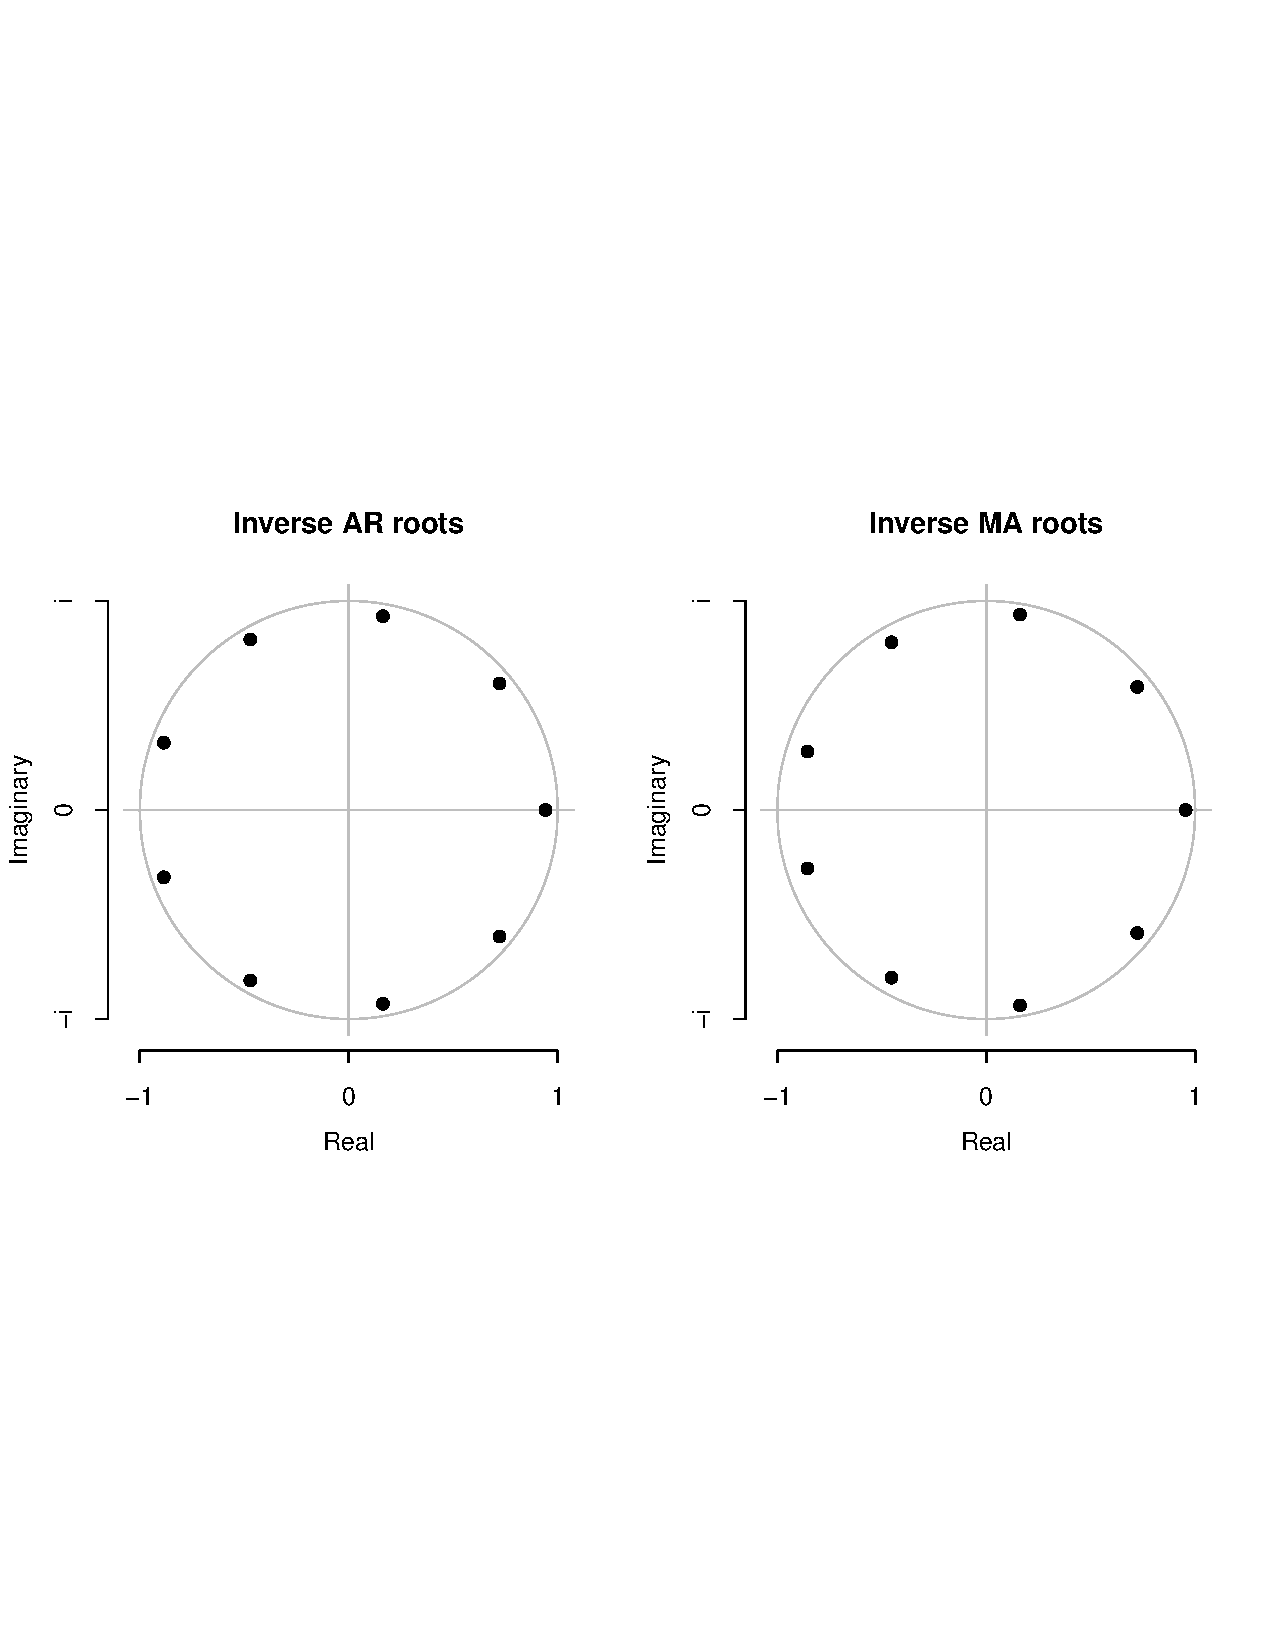
\includegraphics[width=\columnwidth]{figs/Sar1stationary.pdf}
    \caption{Lugar de las raíces para el ARIMA(0,1,9)$\times$SARMA$(1,0)_9$.}
    \label{fig:Inverti3}
\end{figure}

\begin{figure}
    \centering
    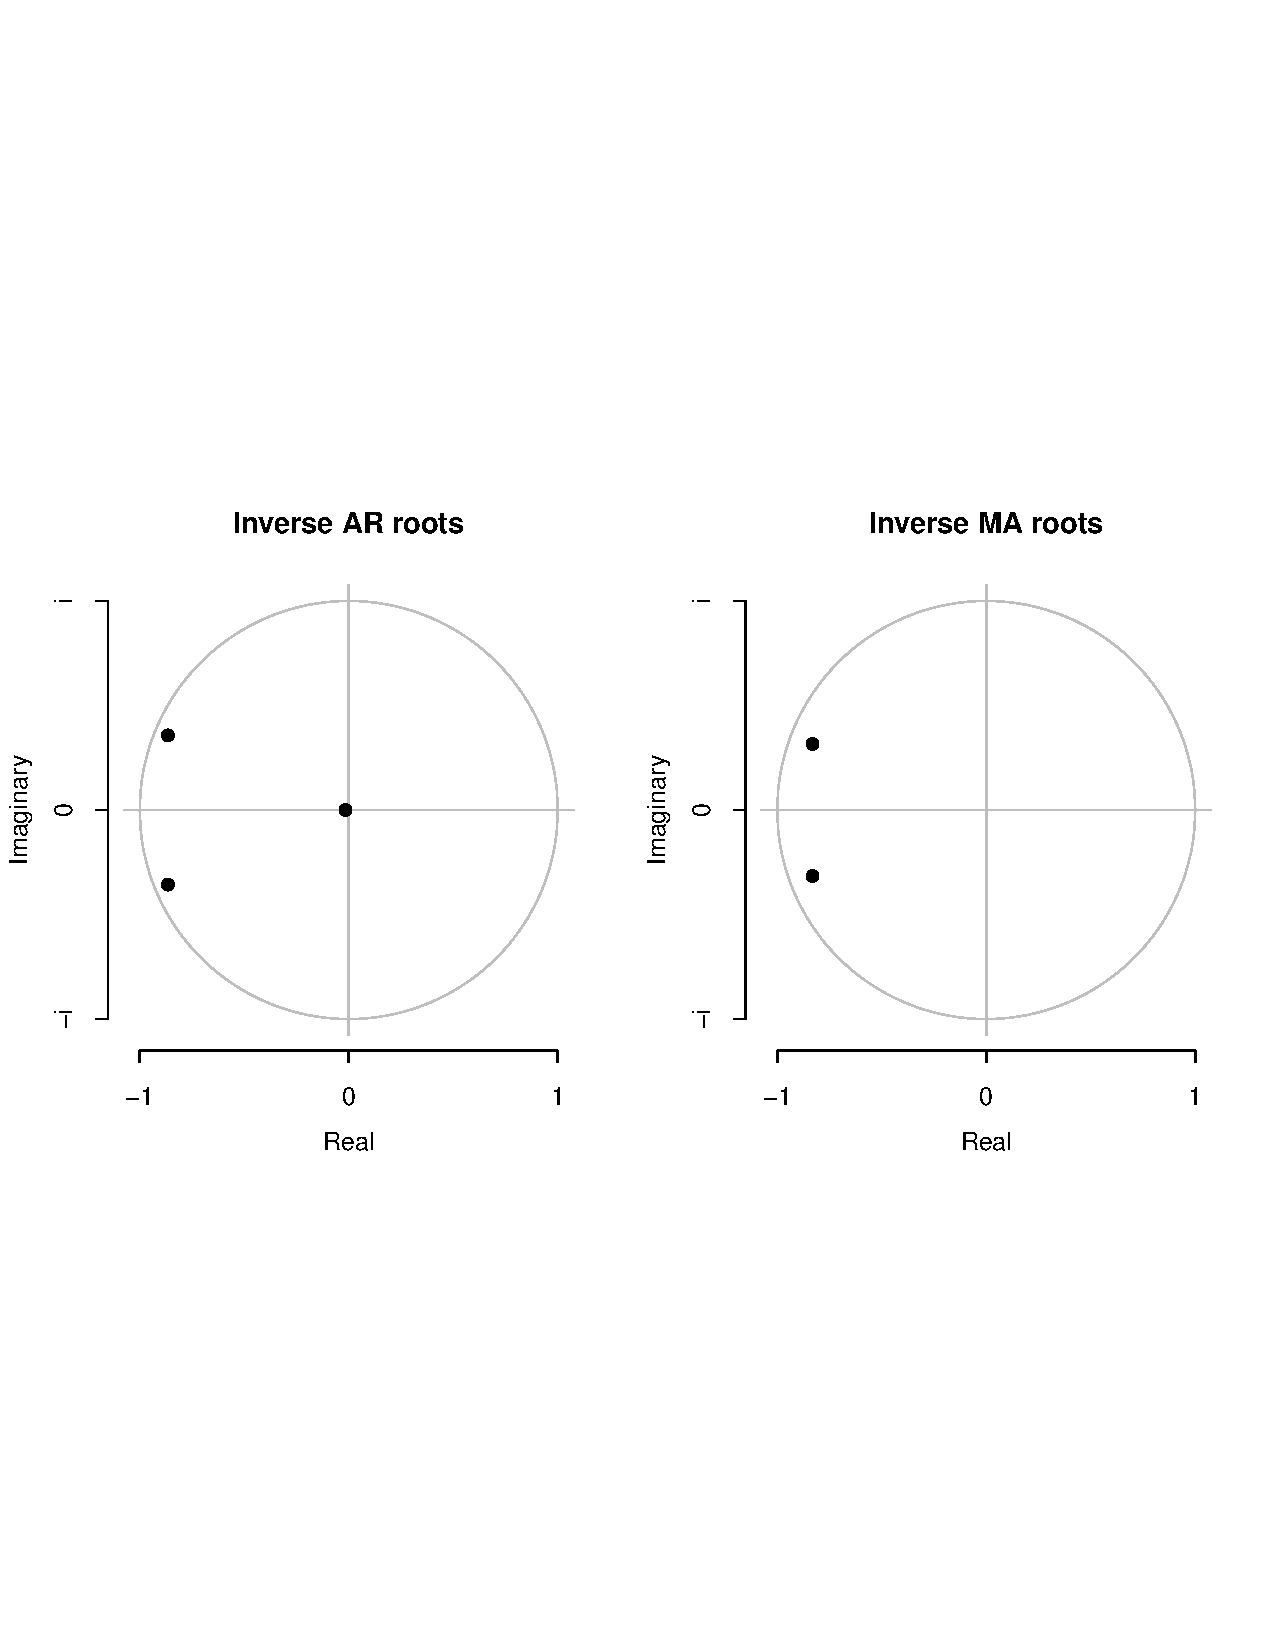
\includegraphics[width=\columnwidth]{figs/Arima312stationarity.pdf}
    \caption{Lugar de las raíces para el ARIMA(3,1,2).}
    \label{fig:Inverti4}
\end{figure}

Para el caso de los modelos GARCH el análisis de estacionariedad y estabilidad esta fuera del alcance de este trabajo. Las gráficas presentadas en las Figuras \ref{fig:Inverti1}-\ref{fig:Inverti4} muestran evidencia de estabilidad e invertibilidad para la mayoría de los modelos, excepto  para el ARIMA(0,1,9)$\times$SARMA(1,0) que tiene dos raíces cercanas a 1 en la parte AR y MA

\subsubsection{Coeficientes significativos} Buscando explicar el más alto porcentaje del comportamiento  de la serie con el menor número de parámetros se estima cada uno de los modelos observando su significancia dentro de la estimación y revisando que no hayan problemas de multicolonealidad (con coeficientes de correlación). La significancia de los coeficientes para cada modelo se presentan en las Tablas \ref{tab:sg_arima919}-\ref{tab:sg_arima312}, y en la Tabla \ref{tab:sg_garch11arma10} se muestra la robustez obtenida para el modelo GARCH.

\begin{table}
\centering
\caption{Significancia de los coeficientes  $\mathrm{ARIMA}(9,1,9)$.}
\label{tab:sg_arima919}
\begin{tabular}{ccc}
\hline
\textbf{Lag} &\textbf{AR} & \textbf{MA} \\ \hline
 1&0.395  & 0.318 \\
 2&0.187  & 0.234 \\
 3&0.779  & 0.820 \\
 4&1.691  & 1.484 \\
 5&0.249  & 0.214 \\
 6&0.065 & 0.137 \\
 7&0.050 & 0.125 \\
 8&1.130  & 0.853 \\
 9&0.314  & 0.508 \\ \hline
\end{tabular}
\end{table}

\begin{table}
\centering
\caption{Significancia de los coeficientes  $\mathrm{ARIMA}(3,1,2)$ con 4 variables exogenas.}
\label{tab:sg_arima312v4}
\begin{tabular}{cccc}
\hline
\textbf{Lag} &\textbf{AR} & \textbf{MA} & \textbf{xreg} \\
\hline
1 & 6.903 & 6.29864 & 1.704 \\
2 & 7.119 & 8.738227 & 0.608 \\
3 & 1.253 & $\times$  & 0.974 \\
4 &  $\times$ & $\times$ & 0.314 \\ \hline
\end{tabular}
\end{table}

\begin{table}
\centering
\caption{Significancifa de los coeficientes  $\mathrm{ARIMA}(0,1,9)$ x $\mathrm{SARMA(1,0)}$.}
\label{tab:sg_arima019xsar1}
\begin{tabular}{ccc}
\hline
\textbf{Lag} &\textbf{MA} & \textbf{SARMA} \\ \hline
1 & 4.123 &  5.957 \\ 
2 & 0.303 & $\times$\\
3 & 0.064 & $\times$\\
4 & 4.199 & $\times$\\
5 & 1.246 & $\times$\\
6 & 0.993 & $\times$ \\
7 & 2.290 & $\times$\\
8 & 2.119 & $\times$\\
9 & 4.864 & $\times$\\
\hline
\end{tabular}
\end{table}

\begin{table}
\centering
\caption{Significancia de los coeficientes  $\mathrm{ARIMA}(3,1,2)$}
\label{tab:sg_arima312}
\begin{tabular}{ccc}
\hline
\textbf{Lag} &\textbf{AR} & \textbf{MA} \\ \hline
1 & 28.353 & 30.509\\
2 & 10.749 & 13.308\\
3 & 0.406& $\times$ \\
\hline
\end{tabular}
\end{table}

\begin{table}
\centering
\caption{Robustes de los coeficientes  $\mathrm{GARCH(1,1)}$ x $\mathrm{ARMA(1,0)}$.}
\label{tab:sg_garch11arma10}
\begin{tabular}{ccc}
\hline
\textbf{Coeficientes} &\textbf{p-valor} \\ \hline
mu & 0.230 \\
ar1 & 0.143 \\
omega & 0.191 \\
alpha1 & 0.054 \\
beta1 & 0.000 \\
gamma1 & 0.832\\
\hline
\end{tabular}
\end{table}
Para el caso de GARCH es de suma importancia evaluar los errores estándar robustos debido a los problemas de heterocedasticidad realizando una corrección por medio de la matriz de varianzas y covarianzas, generando que la media de la serie tenga retornos diarios distintos.

\subsubsection{Bondad de ajuste} Los criterios de información que se usan para la bondad de ajuste se utilizan para escoger entre un posible conjunto de modelos. Se utilizaron: el $R^2$ estándar y los criterios de información de Akaike y Bayes (AIC y BIC respectivamente). Los resultados para la bondad de ajuste se presentan en la Tabla \ref{tab:tablabondadA}.
\begin{table}
\centering
\caption{Criterios de información}
\label{tab:tablabondadA}
\begin{tabular}{cccl}
\hline
\textbf{Modelos} & $R^2$ & \textbf{AIC} & \textbf{BIC} \\ \hline
ARMA(9,1,9) & 0.985 & 4695.638 & 4792.926 \\
ARMA(0,1,9) X SAR(1,0) & 0.985 & 4694.674 & 4750.998 \\
ARIMA(3,2,1) & 0.985 & 4702.508 & 4733.23 \\
ARIMAX(3,2,1) & 0.985 & 4725.072 & 4776.277\\
GARCH(1,1)/ARMA(1,0) & $\times$ & 3.466 & 3.4913
\\ \hline
\end{tabular}
\end{table}

\subsubsection{Predicción}
Debido a que la serie es una acción financiera que tiene valores semanales se decide realizar una predicción para un periodo de 21 días para cada uno de los modelos. Se realizo un proceso de validación cruzada, utilizando los datos reales con el fin de validar si las predicciones son adecuadas.

En la Figura \ref{fig:con medias} se observan las predicciones para el mes de Octubre 2020 para cada modelo. Se puede observar que las predicciones realmente no son adecuadas y a duras penas capturan la dinámica en los primeros periodos. No obstante, esta es la gráfica de la media para las predicciones y no se hizo el análisis con los intervalos de confianza, por lo que es posible que las predicciones estén bien de acuerdo al nivel de los intervalos.

\begin{figure}
    \centering
    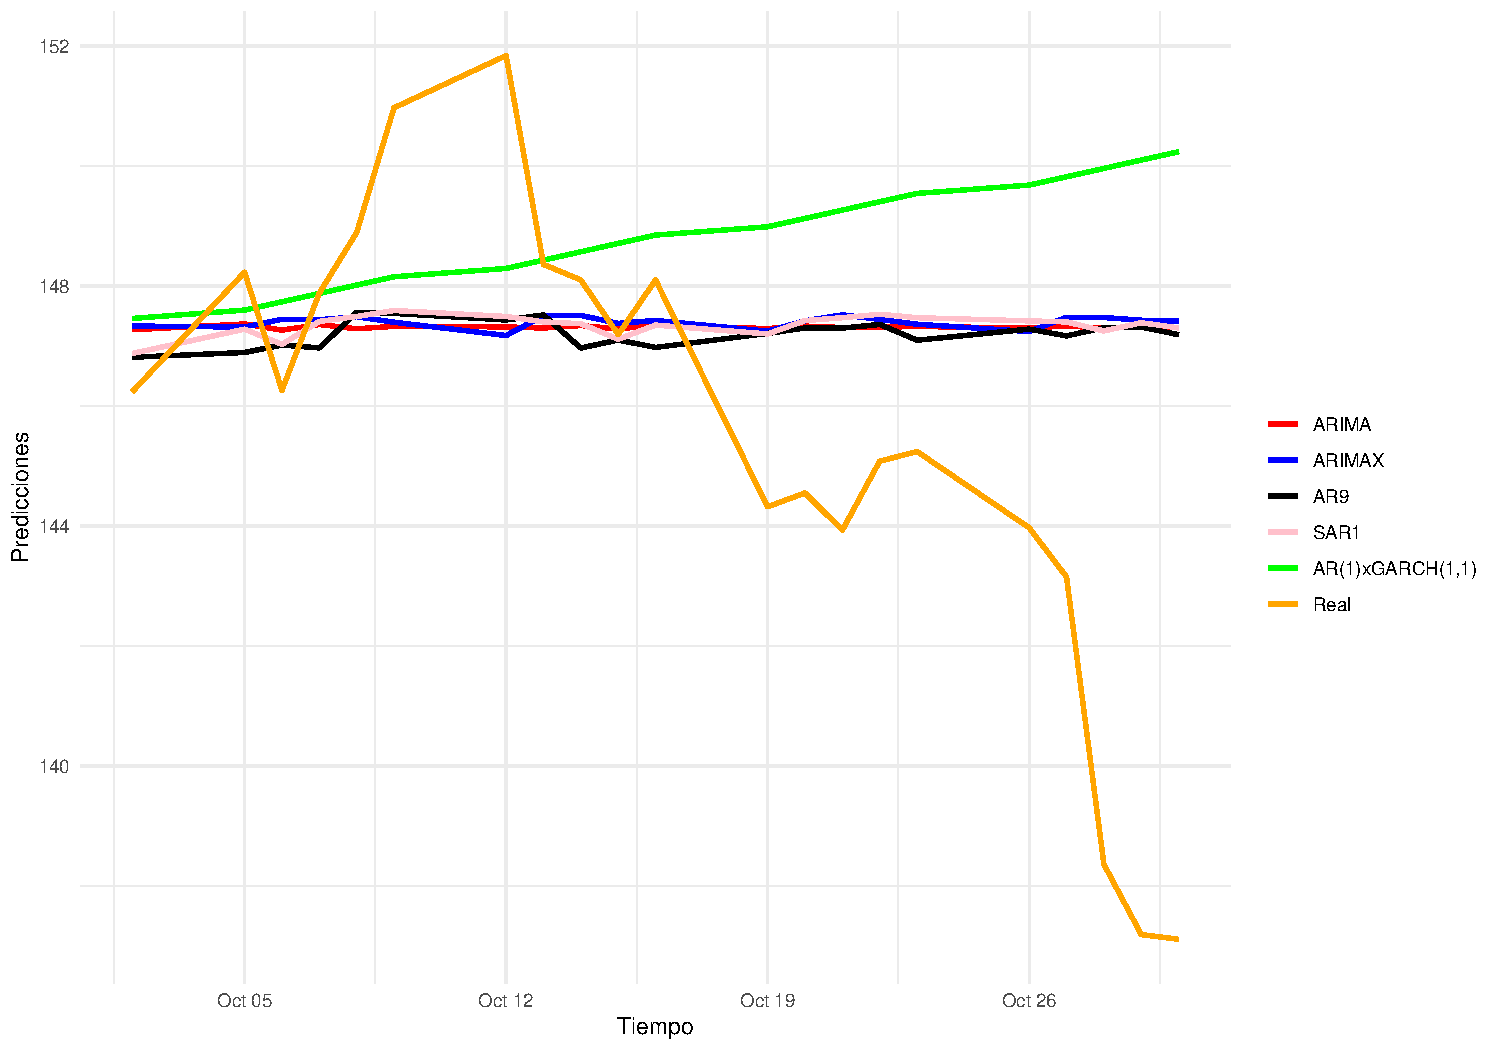
\includegraphics[width=\columnwidth]{figs/forecast.pdf}
    \caption{Predicciones de la media de los modelos }
    \label{fig:con medias}
\end{figure}

Posteriormente, se corrieron predicciones de 1 periodo utilizando los datos reales en el periodo anterior. Las gráficas de cada una de estas predicciones pueden observarse en las Figuras \ref{fig:pred_data_1}-\ref{fig:pred_data_5}. Estos pronósticos a 1 periodo muestran muy buen ajuste con respecto a los datos reales, siendo así que los modelos se podrían utilizar las para predicciones a 1 o máximo 2 periodos.

\begin{figure}
    \centering
    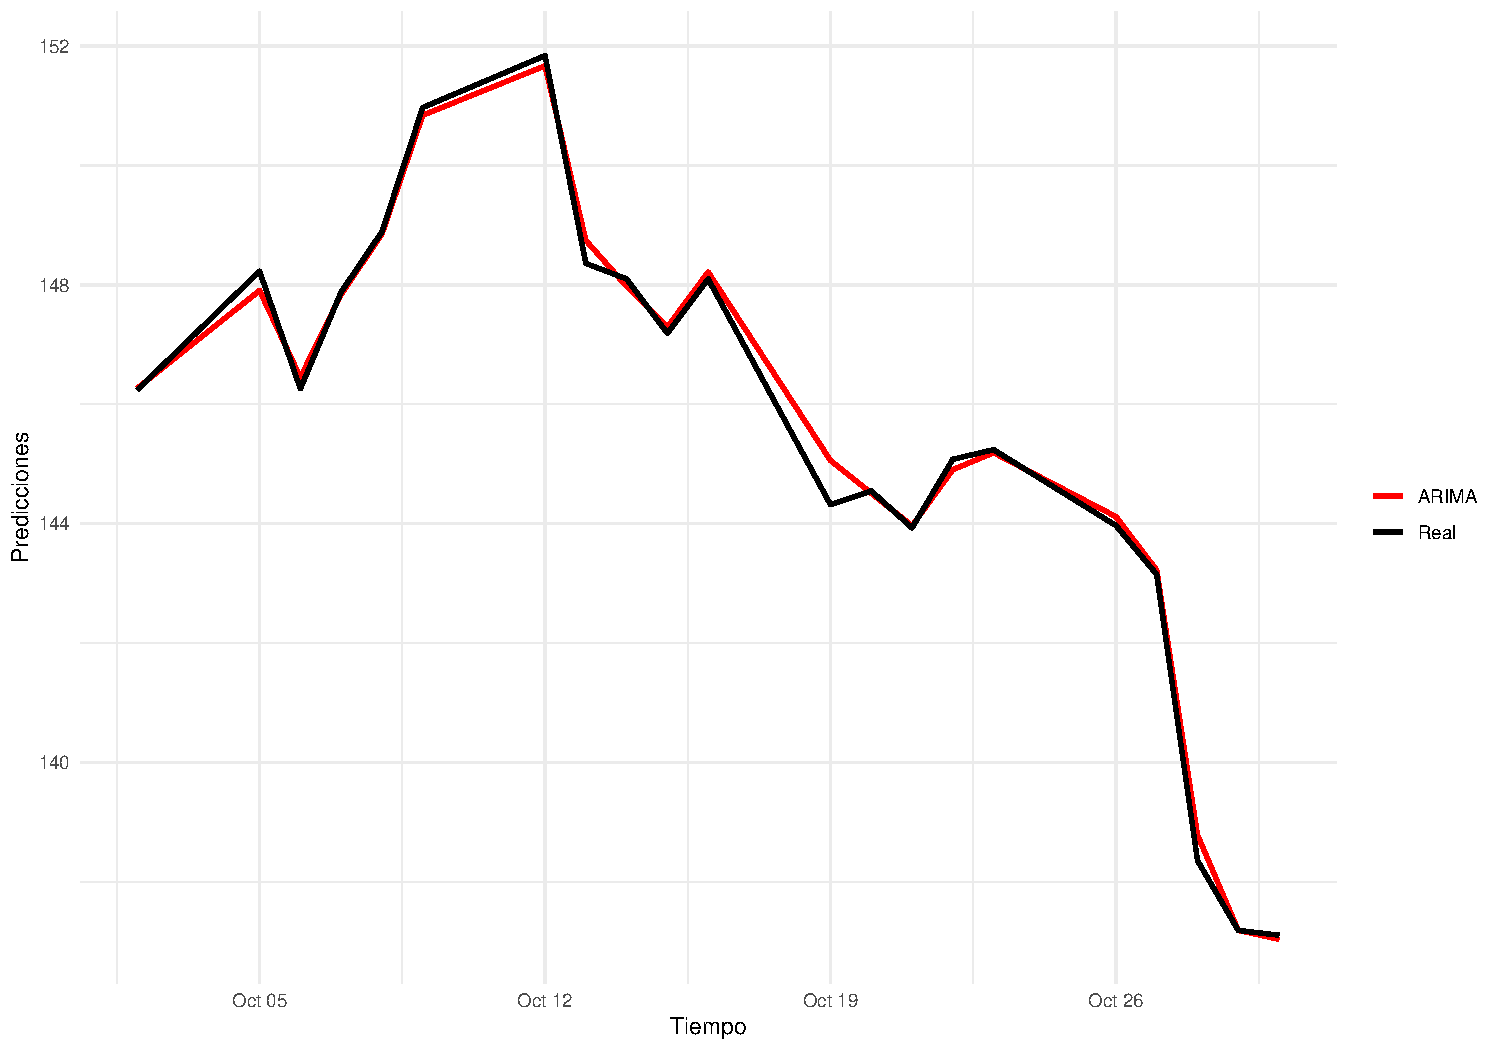
\includegraphics[width=\columnwidth]{figs/all1.pdf}
    \caption{Predicción para ARIMA(3,2,1).}
    \label{fig:pred_data_1}
\end{figure}

\begin{figure}
    \centering
    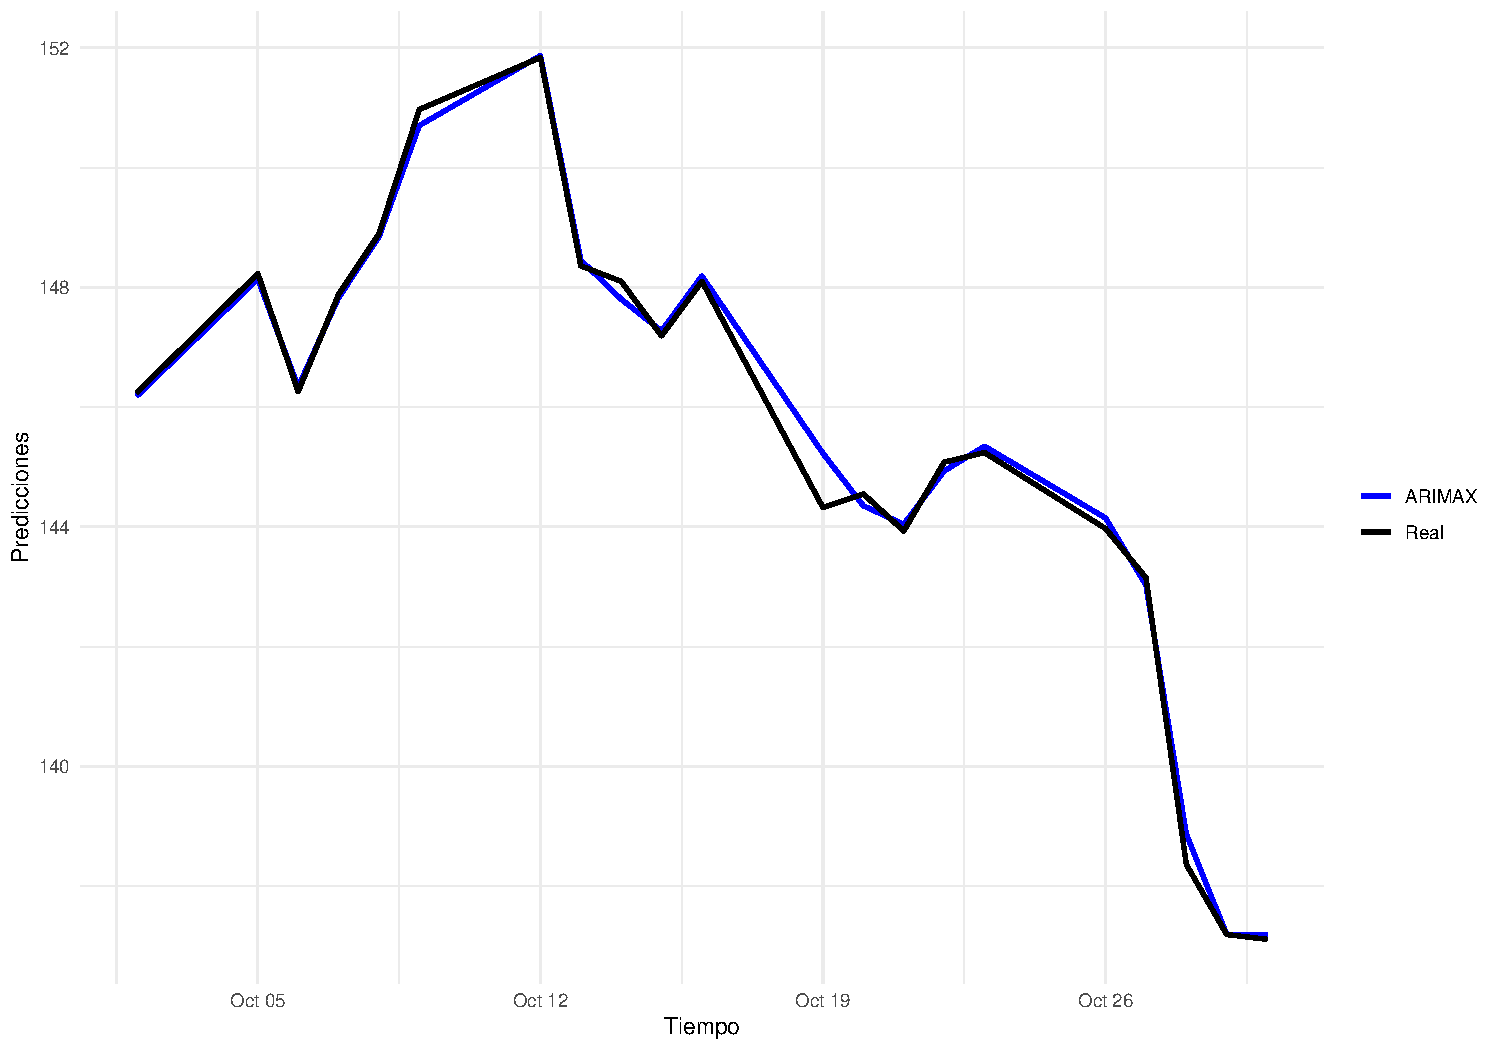
\includegraphics[width=\columnwidth]{figs/all2.pdf}
    \caption{Predicción para ARIMAX(3,2,1).}
\end{figure}

\begin{figure}
    \centering
    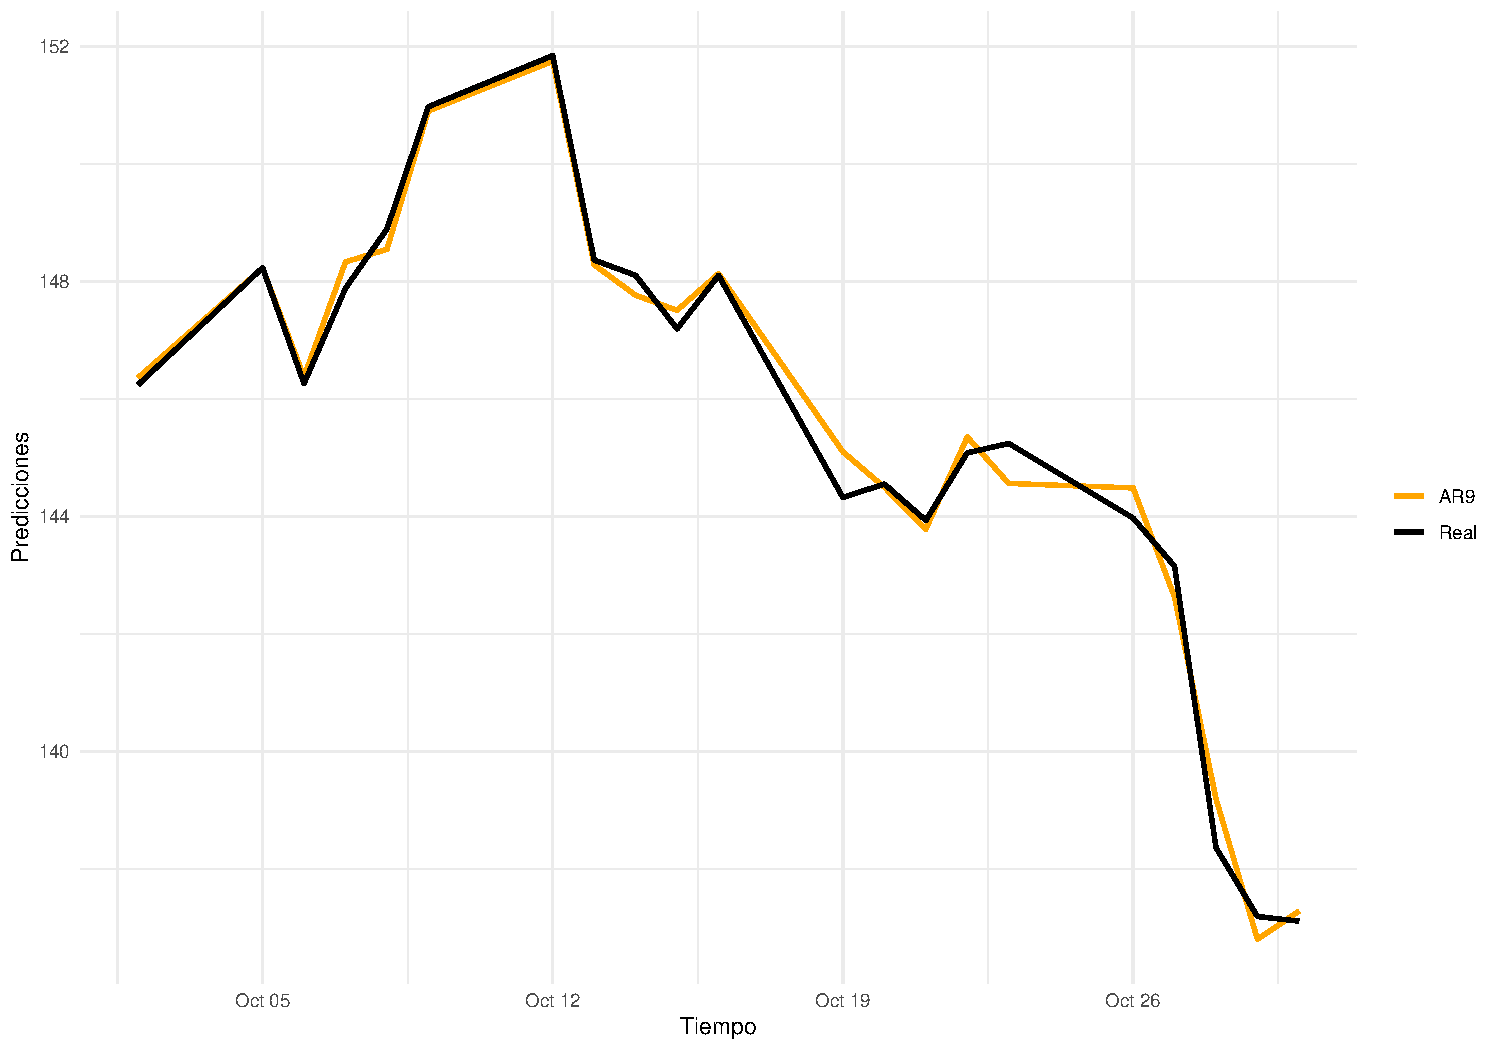
\includegraphics[width=\columnwidth]{figs/all3.pdf}
    \caption{Predicción para ARIMA(9,1,9).}
\end{figure}

\begin{figure}
    \centering
    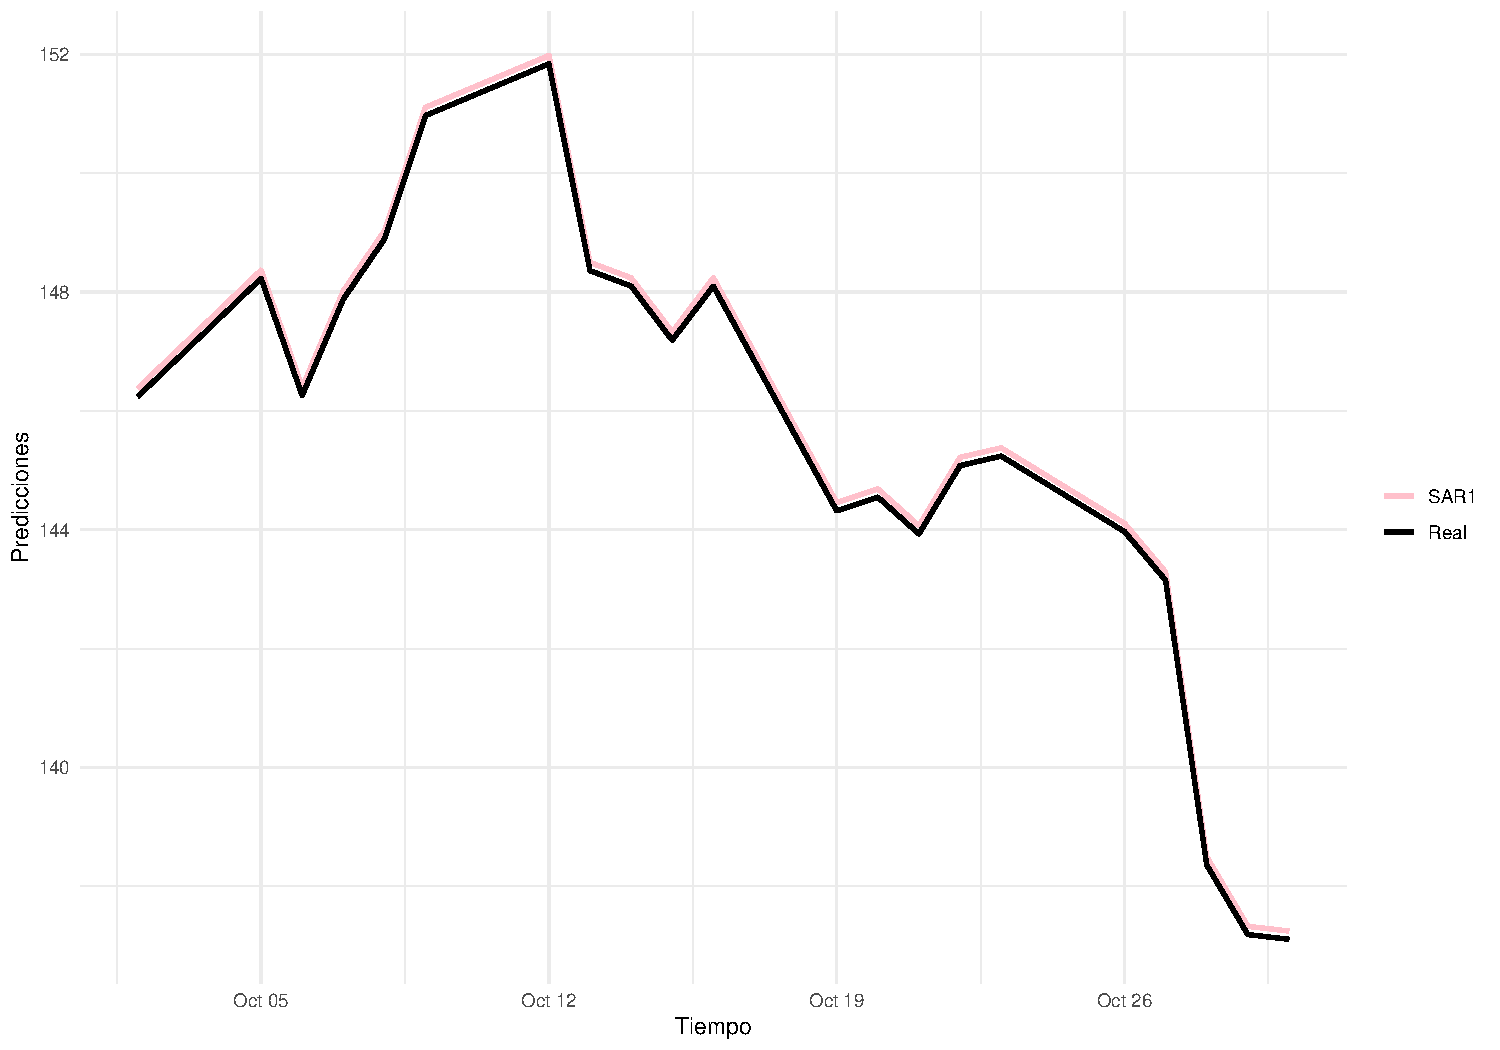
\includegraphics[width=\columnwidth]{figs/all4.pdf}
    \caption{Predicción para SAR1.}
\end{figure}

\begin{figure}
    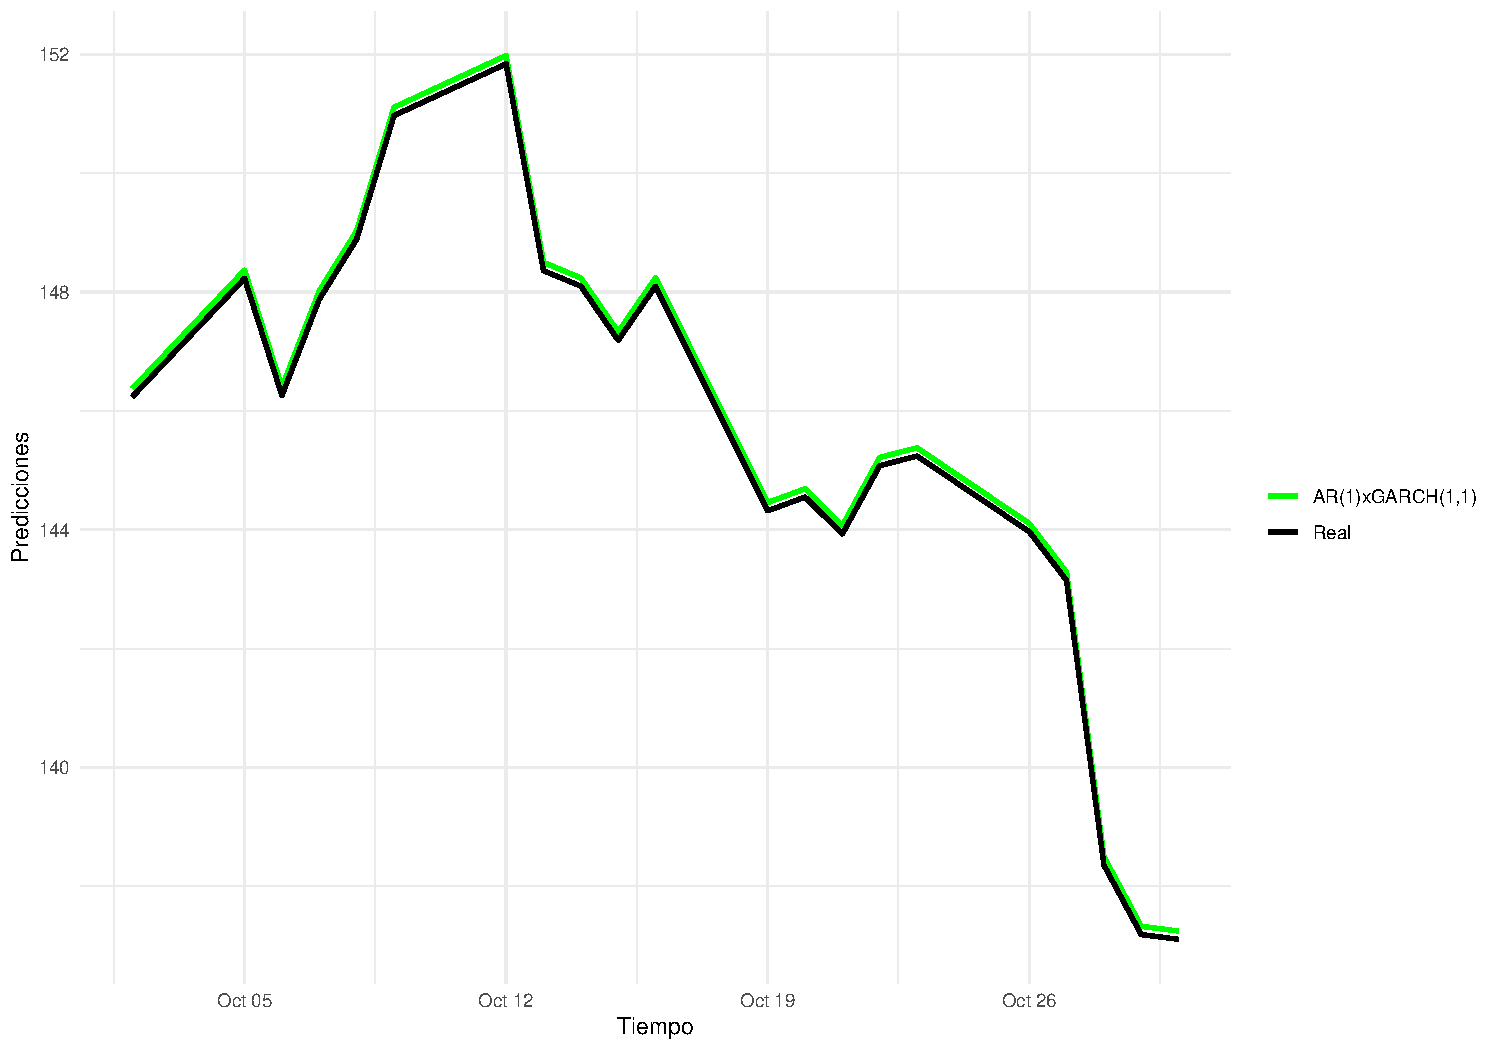
\includegraphics[width=\columnwidth]{figs/all5.pdf}
    \caption{Predicción para GARCH(1,1)/ARMA(1,0).}
    \label{fig:pred_data_5}
\end{figure}

\section{Conclusiones}
Los resultados obtenidos muestran que, aunque los modelos propuestos en general cumplen con los requerimientos de validación, las predicciones obtenidas no son las más adecuadas a largo plazo. Los resultados de las predicciones ``in-sample'' para el mes de Octubre 2020 no se acercan a los valores reales, aún más, no reflejan la rica dinámica evidenciada en los datos reales. 

Por otra parte, se cree que los modelos todavía podrían ser útiles para evaluar la dinámica del proceso generador de datos, pues la mayoría de modelos cumplen con los supuestos para la validación y la predicción utilizando los datos reales es muy buena en general, de donde se puede afirmar que el ajuste el bueno sobre los datos y que las estimaciones siguen siendo útiles para máximo 2 periodos hacia adelante.

Adicionalmente, cabe resaltar que este trabajo es preliminar y meramente exploratorio. Se podrían considerar varios aspectos para futuros trabajos: hacer un trabajo igual de extenso para la exploración de modelos tipo GARCH, puesto que de la literatura se sabe que estos modelos son más adecuados para representar series financieras. También podría considerarse modelos de transición, con impulsos o varios regímenes, para compensar el error que induce el choque en el crecimiento generado por la pandemia en 2020. Finalmente, los autores consideran que una comparación entre modelos de series de tiempo y modelos propios de series financieras (cálculo estocástico) podría ser de gran valor.

\bibliographystyle{IEEEtran}
\bibliography{ref}
\end{document}